%\documentclass[useAMS,usenatbib,fleqn,dvipdfm]{emulateapj-rtx4}
%\documentclass[fleqn,dvipdfmx]{emulateapj-rtx4}
\documentclass[fleqn,dvipdfmx]{article}

%\usepackage[dvipdfm]{graphicx,color}
%\usepackage{amssymb}
\usepackage{amsmath}
%\usepackage{ulem}
\usepackage{bm}
\usepackage{color}
\usepackage{graphicx}

\newcommand{\jcop}{Journal of Computational Physics}
\newcommand{\sci}{Science}

\newcommand{\redtext}[1]{\textcolor{red}{#1}}
\newcommand{\bluetext}[1]{\textcolor{blue}{#1}}

\newcommand{\gcm}{\mbox{g~cm}^{-3}}
\newcommand{\cms}{\mbox{cm s}^{-1}}
\newcommand{\ergs}{\mbox{erg s}^{-1}}
\newcommand{\ergcms}{\mbox{erg cm}^{-2}~\mbox{s}^{-1}}
\newcommand{\cowd}{CO~WD }
\newcommand{\cowds}{CO~WDs }

\newcommand{\mdlx}[1]{$#1$M}
\newcommand{\vej}{v_{\rm ej}}
\newcommand{\tta}{t_{3\alpha}}
\newcommand{\ttar}{t_{3\alpha, {\rm r}}}
\newcommand{\ttas}{t_{3\alpha, {\rm s}}}
\newcommand{\tcc}{t_{\rm cc}}
\newcommand{\tccr}{t_{\rm cc,r}}
\newcommand{\tccs}{t_{\rm cc,s}}
\newcommand{\tdy}{t_{\rm dyn}}
\newcommand{\deta}{\epsilon_{3\alpha}}
\newcommand{\decc}{\epsilon_{\rm cc}}
\newcommand{\fsni}{$^{56}$Ni }
\newcommand{\fhe}{f_{\rm He}}

\newcommand{\km}[1]{{\bf{[KM: #1]}}}

%%%%%%%%%%%%%%%%%%%%%%%%%%%%%%%%%%%%%%%%%%%%%%%%

\begin{document}

\section{SPH w/ artificial conductivity}

Suppose we know acceleration, time derviative of energy, coefficient
viscosity, and the next timestep at the initial time. We integrate
each particle as follows:
\begin{enumerate}
\item Calculate the position, and predict the velocity and
  energy: \label{item:predict}
  \begin{align}
    \bm{r}_{i} &= \bm{r}^{(0)}_i + \bm{v}^{(0)}_i \Delta t +
    \frac{1}{2} \bm{a}^{(0)}_i \Delta t^2, \\
    %%
    \bm{v}^{(1/2)}_i &= \bm{v}^{(0)}_i + \frac{1}{2} \bm{a}^{(0)}
    \Delta t, \\
    %%
    u^{(1/2)}_i &= u^{(0)}_i + \frac{1}{2} \dot{u}^{(0)} \Delta t \\
    %%
    \alpha^{(1/2)}_i &= \alpha^{(0)}_i + \frac{1}{2}
    \dot{\alpha}^{(0)} \Delta t, \\
    %%
    \alpha^{{\rm u},(1/2)}_i &= \alpha^{{\rm u},(0)}_i + \frac{1}{2}
    \dot{\alpha}^{{\rm u},(0)} \Delta t, \\
    %%
    \tilde{\bm{v}}_{i} &= \bm{v}^{(0)}_i + \bm{a}^{(0)}_i \Delta t, \\
    %%
    \tilde{\bm{u}}_{i} &= \bm{u}^{(0)}_i + \dot{\bm{u}}^{(0)}_i \Delta
    t + \epsilon_{{\rm nuc},i}(\Delta t), \\
    %%
    \tilde{\alpha}_i &= \alpha^{(0)}_i + \dot{\alpha}^{(0)}_i \Delta t
    \\
    %%
    \tilde{\alpha}^{\rm u}_i &= \alpha^{{\rm u},(0)}_i +
    \dot{\alpha}^{{\rm u},(0)}_i \Delta t,
  \end{align}
  where ($\epsilon_{{\rm nuc},i}$) is energy generated through nuclear
  reaction. \redtext{(When the reaction is exothermic, the density and
    temperature are fixed at this time. On the other hand, when the
    reaction is endothermic, only the density is fixed at this time.)}

%%%%%%%%%%%%%%%%%%%%%%%%%%%%%%%%%%%%%%%%%%%%%%%%%%%%%%%%%%%%%%%%%%%%%
\item Calculate the density, kernel-support length and grad-h term of
  each particle by an iterative method:
  \begin{enumerate}
  \item Estimate the density by the following
    expression: \label{item:estimatedensity}
    \begin{align}
      \rho_i = \sum_j m_j W_i
    \end{align}
    where $W_i=W(r_{ij},H_i)$, $r_{ij}=|\bm{r}_{ij}|$, and
    $\bm{r}_{ij}=\bm{r}_i-\bm{r}_j$. The kernel function is expressed
    as
    \begin{align}
      W(r,H) = H^{-D} w(r/H).
    \end{align}
    The formula of $w(q)$ is described in Appendix~\ref{sec:kernels}.
  \item Calculate the kernel length as follow:
    \begin{align}
      H_i = \max \left[ C_{H/h} \times \eta \left( \frac{m_i}{\rho_i}
        \right)^{1/D}, H_{\max} \right],
    \end{align}
    where $h$ is the kernel length. Here, $H_{\max}$ is the initial
    distance of the binary separation, or the maximum \texttt{double}
    in the case of the single WD. The values of $\eta$ and $C_{H/h}$
    are described in Appendix~\ref{sec:kernels}.
  \item Return to step~(\ref{item:estimatedensity}) unless this is the
    3rd time.
  \item Calculate divergence and rotation of $\bm{v}$, grad-h term,
    and gravity correction term:
    \begin{align}
      \nabla \cdot \tilde{\bm{v}}_i &= - \frac{1}{\Omega_i \rho_i} \sum
      \tilde{\bm{v}}_{ij} \cdot \left[ m_j \frac{\partial
          W_i}{\partial r_{ij}} \frac{\bm{r}_{ij}}{r_{ij}} \right], \\
%%
      \nabla \times \tilde{\bm{v}}_i &= \frac{1}{\Omega_i \rho_i} \sum
      \tilde{\bm{v}}_{ij} \times \left[ m_j \frac{\partial
          W_i}{\partial r_{ij}} \frac{\bm{r}_{ij}}{r_{ij}} \right],
      \\
%%
      \Omega_i &= 1 + \frac{1}{D} \frac{H_i}{\rho_i} \sum_j m_j
      \frac{\partial W_i}{\partial H_i},
    \end{align}
    The derivatives of the kernel function are as follows:
    \begin{align}
      \frac{\partial W(r,H)}{\partial r} &= H^{-(D+1)} \frac{\partial
        w(r/H)}{\partial (r/H)} \\
%%
      \frac{\partial W(r,H)}{\partial H} &= -H^{-(D+1)} \left[ D w(q)
        + q \frac{\partial w}{\partial q} \right].
    \end{align}
    The formula of $\partial w/\partial q$ is described in
    Appendix~\ref{sec:kernels}.
%%    The $\eta_i$ can be possibly as
%%    \begin{align}
%%      \eta_i = \frac{H_i}{D\rho_i} \frac{1}{\Omega_i} \sum_j m_j
%%      \frac{\partial \phi(r_{ij},H_{ij})}{\partial H}
%%    \end{align}
  \end{enumerate}
  
%%%%%%%%%%%%%%%%%%%%%%%%%%%%%%%%%%%%%%%%%%%%%%%%%%%%%%%%%%%%%%%%%%%%%
\item Calculate ($\bar{A}_i$) and ($\bar{Z}_i$) as follows:
  \begin{align}
    \bar{A}_i &= \frac{1}{\sum_k X_{i,k}/A_k} \\
%%
    \bar{Z}_i &= \bar{A}_i \sum_k \left( \frac{Z_k}{A_k} X_{i,k}
    \right),
  \end{align}
  where $A_k = (4, 12, 16, 20, 24, 28, 32, 36, 40, 44, 48, 52, 56)$,
  and \\ $Z_k = (2, 6, 8, 10, 12, 14, 16, 18, 20, 22, 24, 26, 28)$.
  
%%%%%%%%%%%%%%%%%%%%%%%%%%%%%%%%%%%%%%%%%%%%%%%%%%%%%%%%%%%%%%%%%%%%%
\item Calculate the pressure ($\tilde{P}_i$) and sound speed
  ($\tilde{c}_{{\rm s},i}$) as follows:
  \begin{align}
    P_i &= (\gamma - 1) \rho_i \tilde{u}_i \\
    c_{{\rm s},i} &= \left( \gamma \frac{P_i}{\rho_i} \right)^{1/2},
  \end{align}
  or Helmholtz EOS\redtext{, in which case the temperature
    ($\tilde{T}_i$) is also obtained}.

%%%%%%%%%%%%%%%%%%%%%%%%%%%%%%%%%%%%%%%%%%%%%%%%%%%%%%%%%%%%%%%%%%%%%
\item Calculate the Balsara switch:
  \begin{align}
    f_i &= \frac{|\nabla \cdot \tilde{\bm{v}}_i|}{|\nabla \cdot
      \tilde{\bm{v}}_i| + |\nabla \times \tilde{\bm{v}}_i| + 0.0001
      \tilde{c}_{{\rm s},i} / h_i}.
  \end{align}

%%%%%%%%%%%%%%%%%%%%%%%%%%%%%%%%%%%%%%%%%%%%%%%%%%%%%%%%%%%%%%%%%%%%%
\item Calculate the gravity and its correction
  term: \label{item:gravity2}
  \begin{align}
    \bm{g}_{2,i} &= - \frac{G}{2} \sum_j m_j
    \frac{\bm{r}_{ij}}{r_{ij}} \left[ \frac{\partial
        \phi(r_{ij},H_i)}{\partial r_{ij}} + \frac{\partial
        \phi(r_{ij},H_j)}{\partial r_{ij}} \right], \\
%%
    \phi_i &= \frac{G}{2} \sum_j m_j \left[ \phi(r_{ij},H_i) +
      \phi(r_{ij},H_j) \right] \\
%%
    \eta_i &= \frac{H_i}{D\rho_i} \frac{1}{\Omega_i} \sum_j m_j
    \frac{\partial \phi(r_{ij},H_i)}{\partial H_i},
  \end{align}
  where the potential is expressed as:
  \begin{align}
    \phi(r,H) &= - \frac{1}{\left( r^2 + H^2 C_{H/h}^{-2}
      \right)^{1/2}} \\
%%
    \frac{\partial \phi(r,H)}{\partial r} &= \frac{r}{\left( r^2 + H^2
      C_{H/h}^{-2} \right)^{3/2}}, \\
%%
    \frac{\partial \phi(r,H)}{\partial H} &=
    \frac{HC_{H/h}^{-2}}{\left( r^2 + H^2 C_{H/h}^{-2} \right)^{3/2}}.
  \end{align}

%%%%%%%%%%%%%%%%%%%%%%%%%%%%%%%%%%%%%%%%%%%%%%%%%%%%%%%%%%%%%%%%%%%%%
\item Calculate the hydro acceleration, the time derivative of the
  energy, and one term of the gravity: \label{item:hydro}
  \begin{align}
    \bm{a}_i &= - \frac{1}{2} \sum_j \left(
    \frac{\tilde{P}_i}{\Omega_i \rho_i^2} +
    \frac{\tilde{P}_j}{\Omega_j \rho_j^2} + f_{ij} \Pi_{ij} \right)
    \left[ m_j \left( \frac{\partial W_i}{\partial r_{ij}} +
      \frac{\partial W_j}{\partial r_{ij}} \right)
      \frac{\bm{r}_{ij}}{r_{ij}} \right], \label{eq:momentum} \\
%%
    \dot{u}_i &= \frac{1}{2} \sum_j \left( \frac{\tilde{P}_i}{\Omega_i
      \rho_i^2} + \frac{f_{ij} \Pi_{ij}}{2} \right)
    \left[ m_j \left( \frac{\partial W_i}{\partial r_{ij}} +
      \frac{\partial W_j}{\partial r_{ij}} \right)
      \frac{\bm{r}_{ij}}{r_{ij}} \right] \cdot
    \tilde{\bm{v}}_{ij}, \label{eq:udot0} \\
%%
    \bm{g}_{1,i} &= \frac{G}{2} \sum_j m_j \left[ \left( \eta_i
      \frac{\partial W_{i}}{\partial r_{ij}} + \eta_j \frac{\partial
        W_{j}}{\partial r_{ij}} \right) \frac{\bm{r}_{ij}}{r_{ij}}
      \right], \\    
%%
    \left( \nabla^2 u \right)_i &= \sum_j \frac{u_i - u_j}{\rho_{ij}}
    \left[ m_j \left( \frac{\partial W_i}{\partial r_{ij}} +
      \frac{\partial W_j}{\partial r_{ij}} \right)
      \frac{1}{r_{ij}} \right],
  \end{align}
  where $f_{ij}=(f_i+f_j)/2$, and $\Pi_{ij}$ is an artificial
  viscosity. The artificial viscosity is expressed as follows:
  \begin{align}
    \Pi_{ij} &= - \frac{\tilde{\alpha}_{ij}}{2} \frac{v_{ij}^{\rm sig}
      w_{ij}^0}{\rho_{ij}} \\
%%
    v_{ij}^{\rm sig} &= c_{{\rm s},i} + c_{{\rm s},j} - 3w_{ij}^0 \\
%%
    w_{ij}^0 &= \min \left(w_{ij},0\right) \\
%%
    w_{ij} &= \frac{\bm{r}_{ij} \cdot
      \tilde{\bm{v}}_{ij}}{|\bm{r}_{ij}|}
  \end{align}
  where $\tilde{\alpha}_{ij}=(\tilde{\alpha}_i+\tilde{\alpha}_j)/2$,
  and $\rho_{ij}=(\rho_i+\rho_j)/2$. If we introduce Price's thermal
  conductivity, equation~(\ref{eq:udot0}) can be rewritten as:
  \begin{align}
    \dot{u}_i = &\frac{1}{2} \sum_j m_j \left( \frac{\partial
      W_i}{\partial r_{ij}} + \frac{\partial W_j}{\partial r_{ij}}
    \right) \nonumber \\ 
%%
    &\times \Biggl\{ \frac{\tilde{P}_i}{\Omega_i \rho_i^2} w_{ij} -
    \frac{1}{\rho_{ij}} \left[ \frac{1}{4} f_{ij} \tilde{\alpha}_{ij}
      v_{ij}^{\rm sig} (w_{ij}^0)^2 - \tilde{\alpha}_{ij}^{\rm u}
      v_{ij}^{\rm u,sig} \left( u_i - u_j \right) \right]
    \Biggr\}, \label{eq:udot1}
  \end{align}
  where
  \begin{align}
    v_{ij}^{\rm u,sig} = \left( \frac{| \tilde{P}_i - \tilde{P}_j
      |}{\rho_{ij}} \right)^{1/2}
  \end{align}

%%%%%%%%%%%%%%%%%%%%%%%%%%%%%%%%%%%%%%%%%%%%%%%%%%%%%%%%%%%%%%%%%%%%%
\item Calculate $\dot{\alpha}$ and $\dot{\alpha}^{\rm u}$:
  \begin{align}
    \dot{\alpha}_i &= - \frac{\tilde{\alpha}_i - \alpha_{\rm
        min}}{h_i/(0.25\tilde{c}_{{\rm s},i})} + \max \left[ -(\nabla
      \cdot \tilde{\bm{v}}_i)(\alpha_{\rm max}-\tilde{\alpha}_i), 0
      \right] \\
%%
    \dot{\alpha}^{\rm u}_i &= - \frac{\tilde{\alpha}^{\rm u}_i -
      \alpha_{\rm min}^{\rm u}}{h_i/(0.25\tilde{c}_{{\rm s},i})} +
    \frac{h_i|\nabla^2u|_i}{(u_i+\epsilon^{\rm u})^{1/2}} \left(
    \alpha_{\max} - \tilde{\alpha}^{\rm u}_i \right),
  \end{align}
  where we set $\epsilon^{\rm u}=0.0001u_{0,\min}$.

%%%%%%%%%%%%%%%%%%%%%%%%%%%%%%%%%%%%%%%%%%%%%%%%%%%%%%%%%%%%%%%%%%%%%
\item Correct the velocity and energy:
  \begin{align}
    \bm{v}_i &= \bm{v}^{(1/2)}_i + \frac{1}{2} \bm{a}_i \Delta t \\
    %%
    u_i &= u^{(1/2)}_i + \frac{1}{2} \dot{u}_i \Delta t +
    \epsilon_{{\rm nuc},i}(\Delta t) \\
    %%
    \alpha_i &= \alpha^{(1/2)}_i + \frac{1}{2} \dot{\alpha}_i \Delta
    t, \\
    %%
    \alpha^{\rm u}_i &= \alpha^{{\rm u},(1/2)}_i + \frac{1}{2}
    \dot{\alpha}^{\rm u}_i \Delta t,
  \end{align}
  where $\epsilon_{{\rm nuc},i}(\Delta t)$ has been already obtained
  in step~\ref{item:predict}.

%%%%%%%%%%%%%%%%%%%%%%%%%%%%%%%%%%%%%%%%%%%%%%%%%%%%%%%%%%%%%%%%%%%%%
\item Calculate the next timestep:
  \begin{align}
    \Delta t_{\rm next} = C \min_i \left[
      \frac{C_{H/h}^{-1}H_i}{\max_j \left( v_{ij}^{\rm sig} \right) },
      \left| \frac{u_i^{(0)}}{\dot{u}_i^{(0)}} \right| \right].
  \end{align}  
  \redtext{When nuclear reaction is considered, we should see Raskin
    et al.}

%%%%%%%%%%%%%%%%%%%%%%%%%%%%%%%%%%%%%%%%%%%%%%%%%%%%%%%%%%%%%%%%%%%%%
\item Return to step~1.
\end{enumerate}

\section{SPH w/ IAD}

Between step~\ref{item:gravity2} and \ref{item:hydro}, we calculate a
matrix $\mathcal{C}_i$. The size of the matrix is $D \times D$. The
matrix is expressed as
\begin{align}
  \mathcal{C}_i = \left\{ c_{kl,i} \right\} = \left\{ \tau_{kl,i}
  \right\}^{-1},
\end{align}
The component of the inverse matrix, $\tau_{\ij}$, is written as
\begin{align}
  \tau_{kl,i} = \sum_j \frac{m_j}{\rho_j} x_{k,ij} x_{l,ij} W_i,
\end{align}
where $\bm{r}_ij = (x_{1,ij}, x_{2,ij}, x_{3,ij})$ in 3D.

Furthermore, we replace eqs~(\ref{eq:momentum}) and (\ref{eq:udot0})
(or (\ref{eq:udot1})) with the following equations:
\begin{align}
  \bm{a}_i &= - \sum_j m_j \left( \frac{\tilde{P}_i}{\Omega_i
    \rho_i^2} \bm{A}_{ij} - \frac{\tilde{P}_j}{\Omega_j \rho_j^2}
  \bm{A}_{ji} + f_{ij} \Pi_{ij} \bar{\bm{A}}_{ij} \right) \\
%%
  \dot{u}_i &= \sum_j m_j \bm{v}_{ij} \cdot \left(
  \frac{\tilde{P}_i}{\Omega_i \rho_i^2} \bm{A}_{ij} +
  \frac{f_{ij}\Pi_{ij}}{2} \bar{\bm{A}}_{ij} \right),
\end{align}
where $\bm{A}_{ij}=- \left( \mathcal{C}_i \bm{r}_{ij} \right) W_i$,
and $\bar{\bm{A}}_{ij}=\left( \bm{A}_{ij} - \bm{A}_{ji} \right)/2$.

\section{DISPH}

As the initial condition, we have $m_i$, $\bm{r}_i$, $\bm{v}_i$,
$u_i$, $\alpha_i$, and $H_i$. We integrate each particle in the
following way.
\begin{enumerate}

%%%%%%%%%%%%%%%%%%%%%%%%%%%%%%%%%%%%%%%%%%%%%%%%%%%%%%%%%%%%%%%%%%%
\item We take step~(\ref{item:initial}) at the initial time, and
  step~(\ref{item:predict_disph}) at the other times.

  \begin{enumerate}
%%%%%%%%%%%%%%%%%%%%%%%%%%%%%%%%%%%%%%%%%%%%
  \item \label{item:initial} We calculate a tentative density
    $\tilde{\rho}_i$, such that
    \begin{align}
      \tilde{\rho}_i = \sum_j m_j W_i.
    \end{align}
    Then, we obtain $\tilde{P}_i$ from $\tilde{\rho}_i$ and $u_i$.

%%%%%%%%%%%%%%%%%%%%%%%%%%%%%%%%%%%%%%%%%%%%
  \item \label{item:predict_disph} We predict physical quantities at
    the next time:
    \begin{align}
      \bm{r}_{i} &= \bm{r}^{(0)}_i + \bm{v}^{(0)}_i \Delta t +
      \frac{1}{2} \bm{a}^{(0)}_i \Delta t^2, \\
      %%
      \bm{v}^{(1/2)}_i &= \bm{v}^{(0)}_i + \frac{1}{2} \bm{a}^{(0)}
      \Delta t, \\
      %%
      u^{(1/2)}_i &= u^{(0)}_i + \frac{1}{2} \dot{u}^{(0)} \Delta t, \\
      %%
      \alpha^{(1/2)}_i &= \alpha^{(0)}_i + \frac{1}{2}
      \dot{\alpha}^{(0)} \Delta t, \\
      %%
      \tilde{\bm{v}}_{i} &= \bm{v}^{(0)}_i + \bm{a}^{(0)}_i \Delta t, \\
      %%
      \tilde{\bm{u}}_{i} &= \bm{u}^{(0)}_i + \dot{\bm{u}}^{(0)}_i \Delta
      t + \epsilon_{{\rm nuc},i}(\Delta t), \\
      %%
      \tilde{\alpha}_i &= \alpha^{(0)}_i + \dot{\alpha}^{(0)}_i \Delta
      t, \\
      %%
      \tilde{P}_i &= P^{(0)}_i + \dot{P}_i \Delta t, \\
      %%
      \tilde{H}_i &= H^{(0)}_i + \dot{H}_i \Delta t.
    \end{align}
    We obtain the time derivatives $\dot{P}_i$ and $\dot{H}_i$ as follows:
    \begin{align}
      \dot{P}_i &= - \frac{\partial P_i}{\partial \rho} \rho_i (
      \nabla \cdot \bm{v}_i) + \frac{\partial P_i}{\partial u}
      \dot{u}_i, \\
      %%
      \dot{H}_i &= \frac{H_i}{D} (\nabla \cdot \bm{v}_i).
    \end{align}
  \end{enumerate}

%%%%%%%%%%%%%%%%%%%%%%%%%%%%%%%%%%%%%%%%%%%%%%%%%%%%%%%%%%%%%%%%%%%
\item We derive a volume element iteratively.

  \begin{enumerate}
%%%%%%%%%%%%%%%%%%%%%%%%%%%%%%%%%%%%%%%%%%%%
  \item \label{item:volume} We tentatively obtain a volume element as
    follows:
    \begin{align}
      V_i = \frac{1}{\sum_j (\tilde{P}_j/\tilde{P}_i)^k W_i},
    \end{align}
    where we adopt $k=0.0625$. Here, the kernel function is
    \begin{align}
      W(r,H) = H^{-D} w(r/H).
    \end{align}

%%%%%%%%%%%%%%%%%%%%%%%%%%%%%%%%%%%%%%%%%%%%
  \item We obtain $\tilde{H}_i$ and $\tilde{\rho}_i$ as follows:
    \begin{align}
      \tilde{H}_i    &= C_{H/h} \eta V_i^{1/D}, \\
      \tilde{\rho}_i &= \frac{m_i}{V_i},
    \end{align}
    where the values of $C_{H/h}$ and $\eta$ are seen in
    Appendix~\ref{sec:kernels}.

%%%%%%%%%%%%%%%%%%%%%%%%%%%%%%%%%%%%%%%%%%%%
  \item We calculate $\tilde{P}_i$ from $\tilde{\rho}_i$ and
    $\tilde{u}_i$.

%%%%%%%%%%%%%%%%%%%%%%%%%%%%%%%%%%%%%%%%%%%%
  \item We return step~(\ref{item:volume}) unless this is the 3rd
    time.

  \end{enumerate}

%%%%%%%%%%%%%%%%%%%%%%%%%%%%%%%%%%%%%%%%%%%%%%%%%%%%%%%%%%%%%%%%%%%
\item We calculate some auxiliary variables as follows:
  \begin{align}
    \nabla \cdot \tilde{\bm{v}}_i &= - \frac{1}{\tilde{\rho}_i} \sum
    m_j \tilde{\bm{v}}_{ij} \cdot \left[\frac{\partial W_i}{\partial
        r_{ij}} \frac{\bm{r}_{ij}}{r_{ij}} \right], \\
%%
    \nabla \times \tilde{\bm{v}}_i &= \frac{1}{\tilde{\rho}_i} \sum
    m_j \tilde{\bm{v}}_{ij} \times \left[\frac{\partial W_i}{\partial
        r_{ij}} \frac{\bm{r}_{ij}}{r_{ij}} \right], \\
%%
    \tau_{kl,i} &= \sum_j V_j x_{k,ij} x_{l,ij} W_i,
  \end{align}
  where the derivative of the kernel function is
  \begin{align}
    \frac{\partial W(r,H)}{\partial r} &= H^{-(D+1)} \frac{\partial
      w(r/H)}{\partial (r/H)}.
  \end{align}
  Then, we obtain a matrix $\mathcal{C}_i (=\{c_{kl,i}\})$, which is
  the inverse matrix of $\{\tau_{kl,i}\}$.

%%%%%%%%%%%%%%%%%%%%%%%%%%%%%%%%%%%%%%%%%%%%%%%%%%%%%%%%%%%%%%%%%%%%%
\item We calculate the sound of speed ($\tilde{c}_{{\rm s},i}$) and
  the Balsara switch:
  \begin{align}
    f_i &= \frac{|\nabla \cdot \tilde{\bm{v}}_i|}{|\nabla \cdot
      \tilde{\bm{v}}_i| + |\nabla \times \tilde{\bm{v}}_i| + 0.0001
      C_{H/h} \tilde{c}_{{\rm s},i} / \tilde{H}_i}.
  \end{align}

%%%%%%%%%%%%%%%%%%%%%%%%%%%%%%%%%%%%%%%%%%%%%%%%%%%%%%%%%%%%%%%%%%%%%
\item We calculate the gravity and its correction term:
  \begin{align}
    \bm{g}_{2,i} &= - \frac{G}{2} \sum_j m_j
    \frac{\bm{r}_{ij}}{r_{ij}} \left[ \frac{\partial
        \phi(r_{ij},\tilde{H}_i)}{\partial r_{ij}} + \frac{\partial
        \phi(r_{ij},\tilde{H}_j)}{\partial r_{ij}} \right], \\
%%
    \phi_i &= \frac{G}{2} \sum_j m_j \left[ \phi(r_{ij},\tilde{H}_i) +
      \phi(r_{ij},\tilde{H}_j) \right] \\
%%
    \eta_i &= \frac{\tilde{H}_i}{D\rho_i} \frac{1}{\Omega_i} \sum_j
    m_j \frac{\partial \phi(r_{ij},\tilde{H}_i)}{\partial
      \tilde{H}_i},
  \end{align}
  where the potential is expressed as:
  \begin{align}
    \phi(r,H) &= - \frac{1}{\left( r^2 + H^2 C_{H/h}^{-2}
      \right)^{1/2}} \\
%%
    \frac{\partial \phi(r,H)}{\partial r} &= \frac{r}{\left( r^2 + H^2
      C_{H/h}^{-2} \right)^{3/2}}, \\
%%
    \frac{\partial \phi(r,H)}{\partial H} &=
    \frac{HC_{H/h}^{-2}}{\left( r^2 + H^2 C_{H/h}^{-2} \right)^{3/2}}.
  \end{align}

%%%%%%%%%%%%%%%%%%%%%%%%%%%%%%%%%%%%%%%%%%%%%%%%%%%%%%%%%%%%%%%%%%%
\item We calculate the hydro acceleration, the time derivative of the
  energy, and one term of the gravity:
  \begin{align}
    \bm{a}_i &= - \frac{1}{m_i} \sum_j \left[ \tilde{P}_i V_i^2 \left(
      \frac{\tilde{P}_j}{\tilde{P}_i} \right)^k \bm{A}_{ij} -
      \tilde{P}_j V_j^2 \left( \frac{\tilde{P}_i}{\tilde{P}_j}
      \right)^k \bm{A}_{ji} + m_i m_j f_{ij} \Pi_{ij}
      \bar{\bm{A}}_{ij} \right], \\
%%
    \dot{u}_i &= - \frac{1}{m_i} \sum_j \left[ \tilde{P}_i V_i^2
      \left( \frac{\tilde{P}_j}{\tilde{P}_i} \right)^k
      \tilde{\bm{v}}_j \cdot \bm{A}_{ij} - \tilde{P}_j V_j^2 \left(
      \frac{\tilde{P}_i}{\tilde{P}_j} \right)^k \tilde{\bm{v}}_i \cdot
      \bm{A}_{ji} - \frac{m_i m_j f_{ij} \Pi_{ij}}{2}
      \tilde{\bm{v}}_{ij} \cdot \bar{\bm{A}}_{ij} \right], \\
%%
    \bm{g}_{1,i} &= \frac{G}{2} \sum_j m_j \left[ \left( \eta_i
      \frac{\partial W_{i}}{\partial r_{ij}} + \eta_j \frac{\partial
        W_{j}}{\partial r_{ij}} \right) \frac{\bm{r}_{ij}}{r_{ij}}
      \right],
\end{align}
  where $\bm{A}_{ij}=- \left( \mathcal{C}_i \bm{r}_{ij} \right) W_i$,
  and $\bar{\bm{A}}_{ij}=\left( \bm{A}_{ij} - \bm{A}_{ji}
  \right)/2$. The Balsara switch is $f_{ij} = (f_i + f_j)/2$. The
  artificial viscosity is as follows:
  \begin{align}
    \Pi_{ij} &= - \frac{\tilde{\alpha}_{ij}}{2} \frac{v_{ij}^{\rm sig}
      w_{ij}^0}{\tilde{\rho}_{ij}}, \\
%%
    v_{ij}^{\rm sig} &= \tilde{c}_{{\rm s},i} + \tilde{c}_{{\rm s},j}
    - 3w_{ij}^0, \\
%%
    w_{ij}^0 &= \min \left(w_{ij},0\right), \\
%%
    w_{ij} &= \frac{\bm{r}_{ij} \cdot
      \tilde{\bm{v}}_{ij}}{|\bm{r}_{ij}|},
  \end{align}
  where $\tilde{\alpha}_{ij}=(\tilde{\alpha}_i+\tilde{\alpha}_j)/2$,
  and $\tilde{\rho}_{ij}=(\tilde{\rho}_i+\tilde{\rho}_j)/2$.

%%%%%%%%%%%%%%%%%%%%%%%%%%%%%%%%%%%%%%%%%%%%%%%%%%%%%%%%%%%%%%%%%%%
\item We calculate $\dot{\alpha}$:
  \begin{align}
    \dot{\alpha}_i &= - \frac{\tilde{\alpha}_i - \alpha_{\rm
        min}}{H_i/(0.25C_{H/h}\tilde{c}_{{\rm s},i})} + \max \left[
      -(\nabla \cdot \tilde{\bm{v}}_i)(\alpha_{\rm
        max}-\tilde{\alpha}_i), 0 \right].
  \end{align}

%%%%%%%%%%%%%%%%%%%%%%%%%%%%%%%%%%%%%%%%%%%%%%%%%%%%%%%%%%%%%%%%%%%%%
\item Correct the velocity and energy:
  \begin{align}
    \bm{v}_i &= \bm{v}^{(1/2)}_i + \frac{1}{2} \bm{a}_i \Delta t \\
    %%
    u_i &= u^{(1/2)}_i + \frac{1}{2} \dot{u}_i \Delta t +
    \epsilon_{{\rm nuc},i}(\Delta t) \\
    %%
    \alpha_i &= \alpha^{(1/2)}_i + \frac{1}{2} \dot{\alpha}_i \Delta
    t,
  \end{align}
  where $\epsilon_{{\rm nuc},i}(\Delta t)$ has been already obtained
  in step~\ref{item:predict_disph}.

%%%%%%%%%%%%%%%%%%%%%%%%%%%%%%%%%%%%%%%%%%%%%%%%%%%%%%%%%%%%%%%%%%%%%
\item We calculate the next timestep:
  \begin{align}
    \Delta t_{\rm next} = C \min_i \left[
      \frac{C_{H/h}^{-1}H_i}{\max_j \left( v_{ij}^{\rm sig} \right) },
      \left| \frac{u_i^{(0)}}{\dot{u}_i^{(0)}} \right| \right].
  \end{align}  
  \redtext{When nuclear reaction is considered, we should see Raskin
    et al.}

%%%%%%%%%%%%%%%%%%%%%%%%%%%%%%%%%%%%%%%%%%%%%%%%%%%%%%%%%%%%%%%%%%%%%
\item We return to step~\ref{item:predict_disph}.

\end{enumerate}

\section{Helmholtz EOS}

Coorporate Timmes's EOS. The compositions are 100~\% carbon, 50~\%
carbon and 50~\% oxygen, and will be 100~\% helium.

\appendix

\section{Kernels}
\label{sec:kernels}

\subsection{Cubic spline kernel}

We describe the cubic spline kernel:
\begin{align}
  w(r/H) &= 2^D \sigma \times \left\{
  \begin{array}{ll}
    \left( 1 - 6 q^2 + 6 q^3 \right) & (0 \le q < 1/2) \\
%%
    \left[ 2 (1 - q)^3 \right] & (1/2 \le q < 1) \\
%%
    0 & (q \ge 1)
  \end{array}
  \right. \label{eq:cubicspline0-1} \\
%%
  \frac{\partial w(q)}{\partial q} &= (-6) 2^D \sigma
  \times \left\{
  \begin{array}{ll}
    1/3 & (0 \le q < 1/3) \\
%%
    \left(2q - 3q^2 \right) & (1/3 \le q < 1/2) \\
%%
    (1 - q)^2 & (1/2 \le q < 1) \\
    0 & (q \ge 1)
  \end{array}
  \right., \label{eq:cubicspline0-2}
\end{align}
where $\sigma = 2/3$ (1D), $10/7\pi$ (2D), and $1/\pi$ (3D).

For this kernel, $\eta=1.2$, and $C_{H/h}=2$.

The equations~(\ref{eq:cubicspline0-1}) and (\ref{eq:cubicspline0-2})
can be rewritten as
\begin{align}
  w(r/H) &= 2^D \sigma \times 2 \left[ (1-q)^3_+ - 4 (1/2 - q)^3_+
    \right], \\
%%
  \frac{\partial w(q)}{\partial q} &= (-6)2^D \sigma \times \left[
    (1-q)^2_+ - 4(1/2-q)^2_+ + 3(1/3-q)^2_+) \right],
\end{align}
where $(x)_+ \equiv \max(0, x)$.

\subsection{Wendland C$^2$ kernel}

We describe Wendland C$^2$ kernel: In the case of $D = 1$,
\begin{align}
  w(q) &= C_{\rm W} (1-q)_+^3 (1+3q) \\ \frac{\partial w(q)}{\partial
    q} &= 3 C_{\rm W} \left[(1-q)^3_+ - (1-q)^2_+ (1+3q) \right],
\end{align}
and in the case of $D = 2, 3$,
\begin{align}
  w(q) &= C_{\rm W} (1-q)_+^4 (1+4q) \\ \frac{\partial w(q)}{\partial
    q} &= 4 C_{\rm W} \left[(1-q)^4_+ - (1-q)^3_+ (1+4q) \right],
\end{align}
where $C_{\rm W}=5/4$ ($D=1$), $7/\pi$ ($D=2$), and $21/(2\pi)$
($D=3$). For this kernel, $\eta=1.6$, and $C_{H/h}=1.620185(D=1)$,
$1.897367(D=2)$, and $1.93492(D=3)$.

\subsection{Wendland C$^4$ kernel}

We describe Wendland C$^4$ kernel: In the case of $D = 1$,
\begin{align}
  w(q) &= C_{\rm W} (1-q)_+^5 (1+5q+8q^2) \\
%%
  \frac{\partial w(q)}{\partial q} &= C_{\rm W} (1-q)_+^4 \left[
    -5(1+5q+8q^2) + (1-q)_+ (5+16q) \right]
\end{align}
and in the case of $D = 2, 3$,
\begin{align}
  w(q) &= C_{\rm W} (1-q)_+^6 \left[ 1+6q+(35/3)q^2 \right] \\
%%
  \frac{\partial w(q)}{\partial q} &= C_{\rm W} (1-q)_+^5 \left\{-6
  \left[ 1+6q+(35/3)q^2 \right] + (1-q)_+ \left[ 6+(70/3)q \right]
  \right\}
\end{align}
where $C_{\rm W}=3/2$ ($D=1$), $9/\pi$ ($D=2$), and $495/(32\pi)$
($D=3$). For this kernel, $\eta=1.6$, and $C_{H/h}=1.936492(D=1)$,
$2.171239(D=2)$, and $2.207940(D=3)$.

\section{SPH tests}

\begin{enumerate}
\item 1D shock tube (CUBICSPLINE, USE\_AT1D)
\item 3D shock tube (CUBICSPLINE)
\item Strong shock (CUBICSPLINE, USE\_AT1D)
\item Point like explosion (CUBICSPLINE)
\item Evrard test (CUBICSPLINE, USE\_AT3D, GRAVITY)
\end{enumerate}

\begin{figure}
  \begin{center}
    \includegraphics[width=10cm,bb=0 0 1020 840]{fig/shock_1d/draw.png}
  \end{center}
  \caption{1D shock tube (W2, $\gamma=1.4$, $\alpha=\alpha^{\rm
      u}=1.0$).}
\end{figure}

\begin{figure}
  \begin{center}
    \includegraphics[width=10cm,bb=0 0 1020 840]{fig/shock_3d/draw.png}
  \end{center}
  \caption{3D shock tube (W2, $\gamma=1.4$, $\alpha=\alpha^{\rm
      u}=1.0$).}
\end{figure}

\begin{figure}
  \begin{center}
    \includegraphics[width=10cm,bb=0 0 1020 840]{fig/strong/draw.png}
  \end{center}
  \caption{Strong shock (W2, $\gamma=1.4$, $\alpha=\alpha^{\rm
      u}=1.0$).}
\end{figure}

\begin{figure}
  \begin{center}
    \includegraphics[width=10cm,bb=0 0 1020 840]{fig/pex/draw.png}
  \end{center}
  \caption{Point like explosion (W2, $\gamma=5/3$, $\alpha=\alpha^{\rm
      u}=3.0$).}
\end{figure}

\begin{figure}
  \begin{center}
    \includegraphics[width=14cm,bb=0 0 2120 2000]{fig/evrard/draw.png}
  \end{center}
  \caption{Evrard test (W2, $\gamma=5/3$, $\alpha_{\rm
      min}=\alpha^{\rm u}_{\rm min}=0.1$, $\alpha_{\rm
      max}=\alpha^{\rm u}_{\rm max}=3.0$).}
\end{figure}

\begin{figure}
  \begin{center}
    \includegraphics[width=14cm,bb=0 0 2120 2000]{fig/kh/draw.png}
  \end{center}
  \caption{KH test. Top: W2, $\gamma=5/3$, $\alpha=3, \alpha^{\rm
      u}=0$. Bottom: W2, $\gamma=5/3$, $\alpha=\alpha^{\rm u}=3$. From
    left to right, $t=0$, $t=2\tau_{\rm KH}$, $t=4\tau_{\rm KH}$.}
\end{figure}

\section{EOS tests}

\begin{figure}
  \begin{center}
    \includegraphics[width=14cm,bb=0 0 980 480]{fig/eos/draw.png}
  \end{center}
  \caption{Helmholtz EOS w/ lookup table (top) and w/o (bottom).}
\end{figure}

\begin{figure}
  \begin{center}
    \includegraphics[width=10cm,bb=0 0 520 480]{fig/wdeq/draw.png}
  \end{center}
  \caption{Single COWD equilibrium ($1k/0.1M_{\odot}$) w/ new
    damping. The new damping mode is the addtion of a sort of cooling
    during 100 s, such that $u_{{\rm new},i} = (u_{{\rm old},i} -
    u_{\rm min}(\rho_i)) \exp(-0.1 \Delta t) + u_{\rm min}(\rho_i)$.}
\end{figure}

\begin{figure}
  \begin{center}
    \includegraphics[width=14cm,bb=0 0 880 480]{fig/bwd.1.8_he1e-1/draw.png}
  \end{center}
  \caption{Density and temperature of $1.1M_\odot$ and $1.0M_\odot$
    COWDs ($1k/0.1M_{\odot}$) from $1.8 \times 10^9$cm. Blue points
    indicate helium particles ($f_{\rm He}=0.1$).}
\end{figure}

\begin{figure}
  \begin{center}
    \includegraphics[width=14cm,bb=0 0 880 1200]{fig/wddamp/draw.png}
  \end{center}
  \caption{$1M_\odot$ COWD ($1k/0.1M_{\odot}$).}
\end{figure}

\begin{figure}
  \begin{center}
    \includegraphics[width=14cm,bb=0 0 1000 960]{fig/wddamp/draw2.png}
  \end{center}
  \caption{$1M_\odot$ COWD ($1k/0.1M_{\odot}$).}
\end{figure}

\begin{figure}
  \begin{center}
    \includegraphics[width=14cm,bb=0 0 880 1240]{fig/bwd.1.8/draw.png}
  \end{center}
  \caption{Density and temperature of $1.1M_\odot$ and $1.0M_\odot$
    COWDs ($1k/0.1M_{\odot}$) from $1.8 \times 10^9$cm.}
\end{figure}

\begin{figure}
  \begin{center}
    \includegraphics[width=14cm,bb=0 0 880 1240]{fig/bwd.1.5/draw.png}
  \end{center}
  \caption{Density and temperature of $1.1M_\odot$ and $1.0M_\odot$
    COWDs ($1k/0.1M_{\odot}$) from $1.5 \times 10^9$cm.}
\end{figure}

\begin{figure}
  \begin{center}
    \includegraphics[width=14cm,bb=0 0 880 840]{fig/tempmax/draw.png}
  \end{center}
  \caption{Temperature evolution with mass resolution
    $64k/0.1M_{\odot}$ in the cases of w/ conductivity (top) and w/o
    conductivity (bottom).}
\end{figure}

\begin{figure}
  \begin{center}
    \includegraphics[width=14cm,bb=0 0 880 840]{fig/150928_fin/draw.png}
  \end{center}
  \caption{$\rho$-$T$ and $\rho$-$\bar{A}$ plains with mass resolution
    $64k/0.1M_{\odot}$ in the cases of w/ conductivity (top) and w/o
    conductivity (bottom).}
\end{figure}

\end{document}
